\documentclass{standalone}
\usepackage{tikz}
\usepackage{ctex,siunitx}
\setCJKmainfont{Noto Serif CJK SC}
\usepackage{tkz-euclide}
\usepackage{amsmath}
\usetikzlibrary{patterns, calc,3d}
\usetikzlibrary {decorations.pathmorphing,decorations.pathreplacing,decorations.shapes}
\tikzset{label style/.append style={font=\small}}
\begin{document}
\small
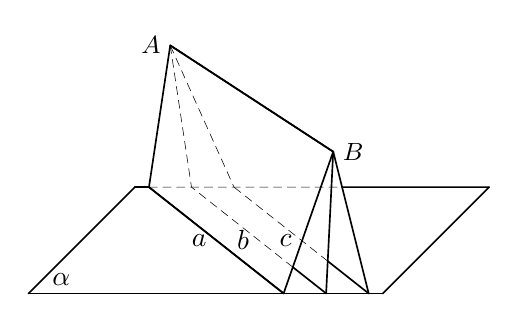
\begin{tikzpicture}[>=latex,scale=0.9]
    \tkzDefPoints{0/0/A',5/0/B',1.5/1.5/D',6.5/1.5/C',4.3/2.0/B,2.0/3.5/A,1.7/1.5/M1,3.6/0/N1,2.3/1.5/M2,4.2/0/N2,2.9/1.5/M3,4.8/0/N3}
    \tkzInterLL(M2,N2)(B,N1)\tkzGetPoint{P}
    \tkzInterLL(M3,N3)(B,N2)\tkzGetPoint{Q}
    \tkzInterLL(C',D')(B,N3)\tkzGetPoint{R}
    \tkzDrawPolygon[semithick](A,M1,N1,B)
    \tkzDrawSegments[semithick](M1,N1 P,N2 Q,N3 A,B B,N2 B,N3 A',B' B',C' M1,D' C',R D',A')
    \tkzDrawSegments[densely dashed](A,M2 A,M3 P,M2 Q,M3 M1,R)
    \tkzLabelLine[pos=0.5,left](M1,N1){$a$}
    \tkzLabelLine[pos=0.5,left](M2,N2){$b$}
    \tkzLabelLine[pos=0.5,left](M3,N3){$c$}
    \tkzLabelAngle[pos=0.5](B',A',D'){$\alpha$}
    \tkzLabelPoints[left](A)
    \tkzLabelPoints[right](B)
\end{tikzpicture}
\end{document}